% !TEX root =  master.tex

\chapter{Grundlagen der Visualisierung}
Das Ziel dieses Projektes liegt in der Erstellung eines hochwertigen Animationsvideos, um den komplexen Sachverhalt der Scheduling Algorithmen von Betriebssystemen intuitiv darzustellen, sodass interessierte Zuschauer relevante Sachverhalte schnell verstehen können. Um für den Lernenden ein Animationsvideo mit möglichst hoher Qualität erstellen zu können, ist eine Beschäftigung mit theoretischen Grundlagen der Visualisierung und Animation unabdingbar. Daher wird im folgenden auf grundlegende Theorien in einer Literaturrecherche eingegangen, welche direkt mit dem von uns produzierten Animationsvideo eingebracht werden. 

Unsere Herangehensweise ein Animationsvideo zu erstellen, wird durch die Dual-Coding-Theorie von Allan Paivio bestätigt, welche besagt, dass Informationen besser verarbeitet und erinnert werden können, wenn diese sowohl visuell als auch verbal präsentiert werden \autocite{paivio_dual_1991}. Diese Theorie wird bei in unserem Animationsvideo umgesetzt, indem neben den visuellen Darstellungen wie Diagrammen oder animierten Algorithmen diese gleichzeitig stets auch auf der Tonspur erklärt werden. Laut der "Cognitive Load Theory" von John Sweller (1988) ist hierbei aber darauf zu achten, dass die kognitive Belastung des Lernenden berücksichtigt wird. Um effektive Bildungsanimationen zu erstellen, ist es entscheidend, die Balance zwischen informativen Inhalten und einer überladenen Darstellung zu finden \autocite{sweller_cognitive_2011}. Durch die sinnvolle Anwendung von Animationen, die komplexe Konzepte in einfachere visuelle Elemente zerlegen, kann das Verständnis erleichtert und die kognitive Belastung reduziert werden. Um den Lernenden daher kognitiv nicht zu überlasten, ist es essentiell, dass animierte Darstellungen stets passend zu der Tonspur sind und diese beiden Komponenten nicht voneinander abweichen. Sollte dies doch der Fall sein, kann dies zu Verwirrung oder kognitiver Leistungsüberschreitung des Lernenden kommen, wodurch die vermittelten Inhalte nicht aufgenommen werden können. 

Um das Animationsvideo einprägsamer für den Lernenden gestalten zu können, ist es sinnvoll die Multimedia-Prinzipien nach Richard E. Mayer (2001) anzuwenden. Diese besagen, dass eine angemessene Kombination von Text, Bildern und Animationen das Lernen deutlich verbessern kann \autocite{mayer_multimedia_2002}. Insbesondere das Kontiguitätsprinzip, das besagt, dass verbundene Text- und Bildinformationen zeitlich und räumlich nahe präsentiert werden sollten, ist für die Gestaltung von Bildungsanimationen relevant. Dies wird direkt in unserem Animationsvideo umgesetzt, wie es in Abbildung \ref{fig:screenshot_text} dargestellt ist. Hier werden mit dezent animiertem Text grafische Vorgänge beschrieben, sodass der Lernende sich diesen Text in Ruhe durchlesen kann ohne bei einer kurzen Unaufmerksamkeit das Verständnis für den gesamten Sachverhalt zu verlieren. 

% Screenshot einfügen mit Beschreibung. Etwas mit Grafik & animiertem Text dazu
\begin{figure}[h]
	\centering
	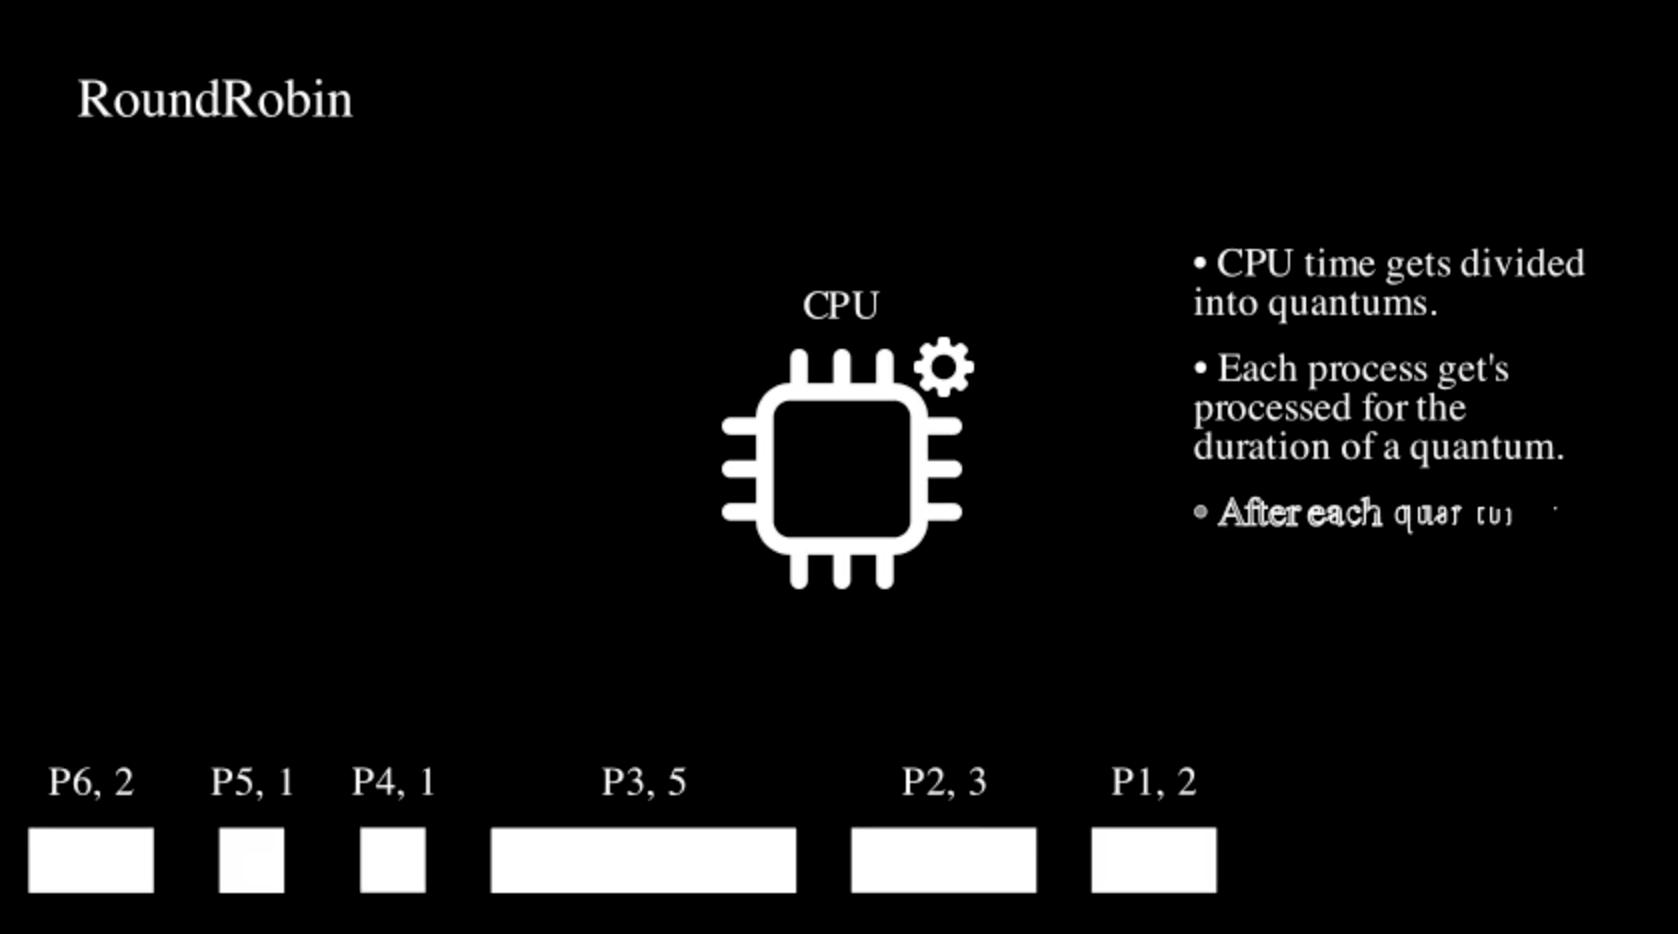
\includegraphics[width=0.8\linewidth]{img/screenshot_text.png} 
	\caption{Die Szene rund um Stelle 00:00min zeigt die Kombination zwischen animierten Bildinformationen mit unterstützendem Text.}
	\label{fig:screenshot_text} 
\end{figure}

Im Kontext von Animationen ist es auch unerlässlich, die Prinzipien der Animation von Disney zu beachten, die von Johnston und Thomas (1981) detailliert beschrieben wurden. Diese Prinzipien, wie "Squash and Stretch" und "Anticipation", sind zwar ursprünglich für die Unterhaltungsanimation entwickelt worden, können jedoch auch in Bildungsanimationen angewendet werden, um Konzepte lebendig und verständlich darzustellen. Beispielsweise kann die Bewegung in einer Animation genutzt werden, um die Dynamik eines mathematischen Prozesses zu verdeutlichen. 

% Screenshot einfügen von "Animation". Wie ein Algorithmus etwas verarbeitet oder so
\begin{figure}[h]
	\centering
	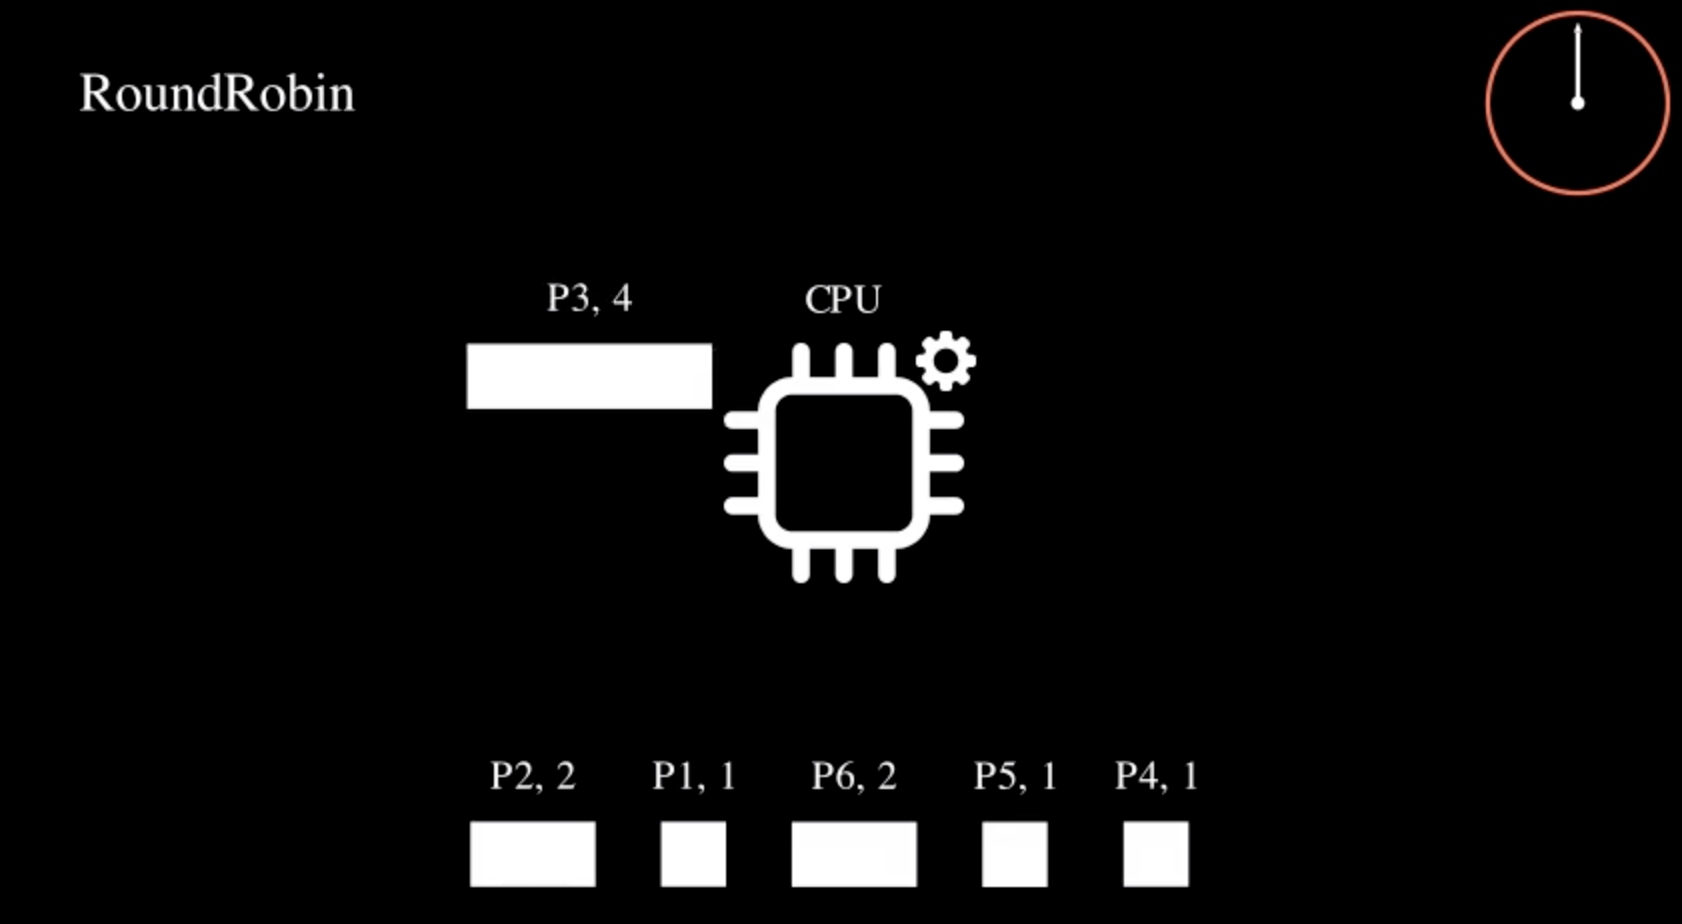
\includegraphics[width=0.8\linewidth]{img/screenshot_animation.png} 
	\caption{Die Szene rund um Stelle 00:00min animierte Darstellung des Round Robin Algorithmus, um komplexe Sachverhalte visuell einfach darzustellen.}
	\label{fig:screenshot_animation} 
\end{figure}

Neben der Wichtigkeit von Animationen ist eine geschickte Auswahl der vorkommenden Farben ebenso essentiell. Laut der Farbtheorie kann die Auswahl von Farben und Kontrasten dabei helfen, wichtige Informationen zu betonen und die visuelle Erfahrung, und somit die vermittelten Inhalte, der Lernenden zu bereichern \autocite{ballard_art_1964}. Auch die Gestaltprinzipien der Wahrnehmung, formuliert von Max Wertheimer (1923), bieten ebenfalls wichtige Einsichten für die Gestaltung von Bildungsanimationen \autocite{wertheimer_untersuchungen_2017}. Diese Prinzipien, wie die Gruppierung von Elementen nach Nähe oder Ähnlichkeit, können genutzt werden, um Beziehungen und Strukturen innerhalb der mathematischen Inhalte zu verdeutlichen. So kann beispielsweise das Prinzip der Nähe dazu verwendet werden, um zu zeigen, wie verschiedene mathematische Elemente miteinander in Beziehung stehen. 